\documentclass{article}
\usepackage{tikz}
\usetikzlibrary{angles,quotes}

\begin{document}

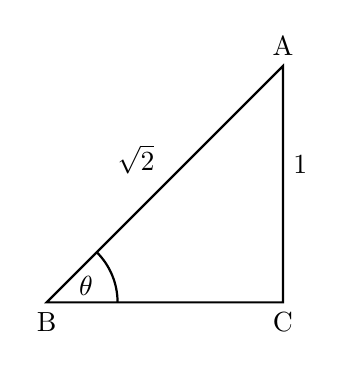
\begin{tikzpicture}[thick]
  % Draw the triangle
  \coordinate (A) at (3,3);
  \coordinate (B) at (0,0);
  \coordinate (C) at (3,0);

  \draw (A) -- (B) -- (C) -- cycle;

  % Add labels
  \node[above] at (A) {A};
  \node[below] at (B) {B};
  \node[below] at (C) {C};
  \draw (1.5, 1.5) node[above left]{$\sqrt{2}$};
  \draw (3.0, 1.5) node[above right]{$1$};

  % Draw angles with markers
  \pic [draw, angle radius=9mm, "$\theta$"] {angle = C--B--A};
\end{tikzpicture}

\end{document}
